\chapter{Úvod}
Při vývoji programů se často můžeme setkat s neuspokojujícími parametry jejich běhu -- ať už z hlediska času běhu nebo využití systémových zdrojů. Přes to, že cena hardware klesá a mzdy programátorů rostou, je často nutné přistoupit k optimalizaci existujícího kódu, namísto prostého přidání systémových prostředků \cite{mooreslaw}\cite{devsalary}. To sice v některých případech pomoci může, nicméně problém neřeší -- pouze jej oddaluje. Pokud chceme podobným problémům v budoucnu předejít a vyhnout se dalším investicím do výkonu, musíme problémový program upravit -- optimalizovat.

Optimalizace může probíhat na několika úrovních. První z možností může být volba efektivnějšího algoritmu -- můžeme zkontrolovat, zda jsme pro řešení problému zvolili vhodný algoritmus a zda neexistuje způsob, jakým bychom mohli dotyčné části řešit efektivněji. Tím je možné, především u vyššího počtu zpracovávaných prvků, dosáhnout výrazně rychlejšího běhu programu samotného. Dále je možné rychlost běhu ovlivnit zefektivněním (či prostou redukcí) přístupů k zařízením (IO), ať už se jedná o práci s diskem nebo síťovou činnost. Dále můžeme optimalizovat na úrovni využití systémových prostředků, typicky paměti (RAM). Právě optimalizaci paměťových nároků se v této práci budu věnovat.

I na snižování množství programem užité paměti lze pohlížet z několika různých úhlů. Navrhovaná řešení se mohou výrazně lišit dosaženými úsporami zdrojů, náročností či finanční nákladností. Jako první můžeme zvážit používané technologie. Změna programovacího jazyku je často natolik drahá, že kompletní přepsání dotyčného software ve většině případů nedává, i přes dosaženou optimalizaci, ekononomický smysl. V rámci námi používaného jazyku tak můžeme, kromě našeho kódu samotného, analyzovat používané frameworky a knihovny. V praxi se můžeme setkat s tím, že závislost na knihovně je přidána pouze z důvodu využití jedné či několika jejích funkcionalit. To je vhodné během vývoje z důvodu rychlosti; později je možné některé z těchto knihoven a jimi poskytované funkce nahradit implementací vlastní a teoreticky tak ušetřit jednotky, desítky či stovky megabytů paměti. Tím ovšem neoptimalizujeme data programu, ale velikost programu samotného.

Na řadu tak přichází právě programová data -- konkrétně datové struktury a typy, které v aplikaci jako její autoři využíváme. A opět je možné k tomuto problému přistoupit z různých úhlů, lišících se pak především hloubkou a důsledností analýzy. Můžeme řešit, zda námi používané typy odpovídají povaze dat -- například, zda rozsah celočíselného typu odpovídá maximální hodnotě dané veličiny.

V praxi mohou být následky nedůsledné optimalizace ještě vážnější. Systémy, které mají obsloužit vysoký počet požadavků za sekundu, je často nutné škálovat -- vytvářet nové, nezávislé jednotky těcho systémů. Ty se poté mohou střídat o příchozí požadavky. Každá neoptimalizace je tedy znásobena počtem těchto instancí. To může naprosto zbytečně zvyšovat náklady na provoz; a to ať už v případě vlastního serveru či cloudových služeb (tzv. serverless).

Cílem této práce je zanalyzovat, k jakým nedostatkům dochází (a zda vůbec) z pohledu neefektivního využití paměti při vývoji Java aplikací. Dále pak vytvořit nástroj, který na tyto nedostatky dokáže poukázat a uživateli napovědět, jakým způsobem by mohl použité prostředky svého programu redukovat a jeho běh tedy optimalizovat. Korektní fungování vytvořeného nástroje bude ověřeno na testovací aplikaci z pohledu správnosti a úplnosti výsledků. Následně pak také prověřeno na větších, rozšířených a běžně používaných Java aplikacích, za účelem posouzení efektivity použití nástroje v praxi, případně také v komerční sféře.



% =====================================================================================================================================================================================



\chapter{Problém správy paměti}
Při vytváření programu má jeho autor na výběr ze dvou způsobů správy paměti -- spravované automaticky (typicky mechanismem typu \zkratka{GC} apod.) či manuálně, případně kombinací těchto přístupů. Ne každý jazyk nabízí oba -- typicky je k dispozici pouze jeden z přístupů, často je správa GC vynucena. Vzhledem k tomu, že majorita nejpopulárnějších programovacích jazyků za poslední roky se řadí mezi vysokoúrovňové, na toto vynucení \zkratka{GC} narazíme u většiny z nich, včetně Javy \cite{stackoverflowinsights}\cite{tiobeindex}. Výjimkou jsou populární nízkoúrovňovější jazyky typu C a C++.

\section{Garbage collector}
\zkratka{GC} je nástroj, starající se o správu paměti programu -- její přidělování, kontrolu a následné uvolnění, ať už pokud je jí málo a je zapotřebí jinde, v pravidelných intervalech nebo při jiných událostech. \zkratka{GC} je obecný termín, tj. neodkazuje na žádnou konkrétní implementaci a způsob chování. Často je v rámci jednoho jazyka (respektive běhového prostředí) zároveň implementováno hned několik algoritmů \zkratka{GC} a dle okolností je vybrán ten nejefektivnější a v danou chvíli nejvhodnější z nich. Některé algoritmy tak mohou běžet velmi rychle bez minimálního zásahu do běhu programu, zatímco jiné vyžadují pro svůj běh o něco delší čas. Často tak je nutné všechen běh kódu pozastavit; v takových případech toto spuštění \zkratka{GC} nazýváme \textit{stop-the-world} (\uv{zastavení světa}, běhu). Pro program je toto zastavení transparentní.

Obecně \zkratka{GC} funguje tak, že si udržuje seznam referencí na jednotlivé objekty, respektive jejich počet. Pokud je některý z objektů dále nereferencovaný, při dalším běhu \zkratka{GC} bude jím zabíraná paměť uvolněna. Nereferencovaným objektem rozumíme, že je nedosažitelný -- nikdo na něj neukazuje. K takovým případům samozřejmě může docházet i v případě jazyků, které fungují bez \zkratka{GC}, např. \texttt{C}. Pokud daný jazyk nezná jiný způsob, jak se k dané paměti opětovně dostat, dochází k tzv. \textit{memory leakům}, tedy únikům paměti. V případě například výše zmíněného \texttt{C} nelze definitivně rozhodnout o nedostupnosti paměti -- díky ukazatelové aritmetice je možné paměť zpětně dopočítat i v případě, že v jednom časovém okamžiku na něj žádný ukazatel v paměti programu neukazuje. Java koncept ukazatelové aritmetiky nezná, po odstranění poslední reference si tedy můžeme být jisti, že už znovu referencovat nikdy nepůjde. V souvislosti s \textit{memory leaky} je nutné zdůraznit, že v tomto případě mám na mysli odstranění poslední reference v rámci paměti uživatelského programu. \zkratka{JVM}, který paměť spravuje, adresu objektu stále zná a je tak schopný jej v rámci běhu \zkratka{GC} odstranit.


% =====================================================================================================================================================================================

\chapter{Struktura paměti programu}

Abychom mohli hledat v paměti a analyzovat nedostatky v rámci jejího využití, musíme nejprve porozumět její struktuře, různým typům oblastí a objektům v nich uložených. Přestože se mnoho následujících konceptů a pravidel vztahuje na ostatní jazyky (a v některých případech i na paměť spravovanou samotným operačním systémem), budu se primárně zaměřovat Javu. Specifikace \zkratka{JVM} neobsahuje žádnou konkrétní podobu paměti či její rozložení, stejně tak jako nespecifikuje žádný konkrétní algoritmus \zkratka{GC} a žádné optimalizace, které se mají nad běžícím kódem vykonávat. Tyto implementační detaily jsou ponechány na možnostech a tvůrčích schopnostech vývojářů, kteří standard implementují. Prostým požadavkem tak je korektní načtení dat ze souboru \texttt{class} a validní vykonání příslušných instrukcí.

\zkratka{JVM}, stejně jako většina ostatních běhových prostředí a jazyků, rozeznává dva druhy datových typů -- primitivní a referenční. Proměnné primitivního typu tak obsahují přímo danou hodnotu, zatímco proměnné referenčních typů referencují (tj. ukazují na) jinde umístěnou paměť, v níž se nachází objekt.

Primitivních datových typů je v Javě několik druhů, konkrétně:

\begin{itemize}
	\item numerické
	\begin{itemize}
		\item celočíselné
			\begin{itemize}
				\item \texttt{byte}
				\item \texttt{short}
				\item \texttt{int}
				\item \texttt{long}
				\item \texttt{char}
			\end{itemize}
		\item s plovoucí desetinnou čárkou
			\begin{itemize}
				\item \texttt{float}
				\item \texttt{double}
			\end{itemize}
		\end{itemize}
	\item \texttt{boolean}
	\item \texttt{returnAddress}
		\begin{itemize}
			\item Speciální datový typ, sloužící jako pointer na \texttt{JVM} instrukce, konkrétně \texttt{jsr}, \texttt{ret} a \texttt{jsr\_w}. V běžném programu jej nicméně nemůžeme jako vývojáři použít ani modifikovat; \texttt{JVM} jej však zná a využívá.
		\end{itemize}
\end{itemize}

Referenční datové typy jsou potom následující:

\begin{itemize}
	\item \texttt{class}
	\item \texttt{array}
	\item \texttt{interface}
\end{itemize}

Typ \texttt{array}, tedy pole, samozřejmě obsahuje seznam prvků určitého typu -- ten nazýváme typem komponenty. Proměnná referenčního typu je ukazatelem do paměti -- místa, kde je obsah objektu umístěn. Prázdný ukazatel, který nereferencuje žádné místo v paměti, nazýváme \texttt{null}. Tato hodnota je výchozí pro všechny proměnné referenčního typu, dokud jim není přiřazena hodnota \cite{jvms}. 

V násedujících odstavcích popisuji různé části paměti \texttt{JVM} -- viz obrázek \ref{obr-jvms-img}.

\section{JVM zásobník}
V případě, že v Javě mluvíme o zásobníku (stack), typicky máme na mysli \zkratka{JVM} zásobník. Kromě něj totiž ještě existuje nativní zásobník, který je vytvořený operačním systémem pro potřeby \zkratka{JVM} samotného. Kromě toho je využívaný i pro některé nízkoúrovňovější činnosti. \zkratka{JVM} stack je spravovaný běhovým prostředím samotným a slouží pro potřeby aplikací, které v rámci prostředí běží.

Pro každé vlákno aplikace je vytvořený zásobník. Do něj jsou ukládány lokální proměnné, hodnoty parametrů metod a návratové hodmoty. Rovněž se stará o volání metod, respektive o návrat do volací metody po zavolání metody jiné. Stejně jako v jiných jazycích (třeba C) je paměť lokálních proměnných automaticky uvolněna při odebírání hodnot ze zásobníku. Takto alokovanou paměť tak není nutné spravovat \zkratka{GC} (či v případě C ručně uvolňovat).

Právě velikost \zkratka{JVM} zásobníku je často omezující faktor při vývoji, na který v některých případech (např. nesprávně zastavovaná rekurze) narážíme. Jeho velikost můžeme nastavit jako parametr při spuštění programu -- konkrétně \texttt{Xss} (respektive \texttt{-XX:ThreadStackSize}). Jeho výchozí velikost je závislá na velikosti dostupné (virtuální) paměti. V souvislosti s nedostatkem paměti a velikostí zásobníku se můžeme setkat se dvěma typy výjimek. \texttt{StackOverflowError} je vyhozena v případě, že během výpočtu narazíme na horní hranici velikosti zásobníku. \texttt{JVM} se případně může pokusit velikost dynamicky zvýšit. Pokud však během této operace narazí na velikost výše zmíněné paměti (což je už limitace nastavená operačním systémem a případně i hardwarovou konfigurací), je vyhozena výjimka jiná -- \texttt{OutOfMemoryError}. Tato výjimka je rovněž produkována v případě, že ručně nastavíme velikost zásobníku takovou, že při jeho vytváření \texttt{JVM} narazí na limity paměti rovnou.

\subsection{Rámce}
Rámce (\textit{frame}) přísluší právě jednomu zásobníku. Data v zásobníku jako takovém jsou totiž neměnná; jsou pouze přidávány/odebírány odkazy na rámce. V každém okamžiku je pro jedno vlákno aktivní právě jeden rámec. 

\subsubsection{Lokální proměnné}
Každý rámec obsahuje pole s lokálními proměnnými. Vzhledem k tomu, že je rámec vytvořen a vložen do \zkratka{JVM} zásobníku při volání metody a znovu odebrán a zničen při návratu z ní, právě toto pole zajišťuje uvolnení paměti alokovaných proměnných. Kromě promenných primitivního typu jsou v tomto poli uloženy rovněž reference na objekty v haldě (viz dále), jejich uvolnění sníží počet referencí na daný objekt a v případě dosažení nulové hodnoty je tento objekt připraven na uvolnění pomocí \zkratka{GC}.

\subsubsection{Zásobník operandů}
Tento zásobník slouží pro mezivýpočty při provádění operací, převážně matematických.

\section{Program counter registr}
\textit{Program counter} (PC) je registr s adresou ukazující na operaci, která se má provést. Vzhledem k tomu, že Java umožňuje vícevláknový běh, má samozřejmě každé vlákno svůj PC. 

\section{Zásobník nativních metod}
Pokud má daná implementace \zkratka{JVM} podporovat i tzv. \texttt{native} metody, měla by obsahovat i zásobník nativních metod. Zdůrazňuji, že \textit{měla} -- specifikace zde benevolentně ponechává rozhodnutí na konkrétním řešení a tento zásobník nutně nevynucuje. Díky konceptu nativních metod je možné přímo z Javy volat kód napsaný např. v C. 

Stejně jako \zkratka{JVM} zásobník, i zásobník nativních metod v některých případech produkuje výjimky. Toto chování je totožné pro oba zásobníky; stejně tak typy těchto chybových stavů jsou stejné.

\section{Halda}
Halda, tj. \textit{heap}, je část paměti, která je pro všechna vlákna programu společná a v Javě tomu není jinak. Díky tomu, že jsou všechny objekty alokovány právě na haldě, k nim můžeme přistupovat napříč metodami, objekty i vlákny. Díky tomu, že platnost v ní umístěných objektů není omezena žádným blokem platnosti (snad jen s výjimkou běhu programu samotného), nedojde k uvolnění jimi zabírané paměti automaticky při opuštění tohoto bloku tak, jak je tomu v případě zásobníku. Právě kvůli tomu nad haldou operuje \zkratka{GC}, který nepotřebné objekty vyhledává a jejich paměť uvolňuje.

Kromě alokovaných objektů jsou rovněž v haldě uchovávány instanční proměnné. Právě z toho důvodu je nutné si dávat pozor na souběh při běhu ve více vláknech --  všechna při přístupu k instanční proměnní manipulují se stejným objektem.

I halda má samozřejmě omezenou velikost. Ta se dá nastavit dvěma přepínači:

\begin{itemize}
	\item \texttt{Xms} -- Výchozí velikost haldy, s kterou Java nastartuje.
	\item \texttt{Xmx} -- Maximální velikost.
\end{itemize}

V případě 32 bitového systému jsou horní hranicí pro maximální velikost haldy 4 Gb, stejně jako v případě velikosti RAM (bez použití různých triků a rozšíření, jako třeba \textit{PAE}, apod.). Jak vyplývá z existence výše zmíněných přepínačů, \zkratka{JVM} dokáže s velikostí haldy dynamicky manipulovat. Program, respektive prostředí pro něj, tak spustí s výchozí hodnotou velikosti a v případě potřeby ji rozšiřuje (nebo naopak zmenšuje) až do maxima. Pokud si běh programu žádá více paměti v haldě, než může \zkratka{JVM} alokovat (tj. než má od systému k dispozici), vyhod, stejně jako v případě zásobníku, výjimku \texttt{OutOfMemoryError}. 

Halda je rozdělena dále do několika prostorů, jak je popsáno dále v kapitole \ref{memory-management}.

\section{Non-heap oblast}
Kromě oblasti metod bsahuje pomocná data, která jsou potřeba pro interní zpracování a potřeby. 
\subsection{Oblast metod}
Oblast, která uchováva data jednotlivých metod. Pro každou načtenou třídu uchovává strukturu se seznamem metod, statickými proměnnými a kódem metod a konstruktorů. Na jednu ze struktur třídy směřuje ukazatel z aktuálně zpracovávaného rámce v zásobníku, pomocí kterého může aktuálně vykonávaný kód přistupovat ke statickým členům třídy.

\begin{figure}[h]
	\centering
	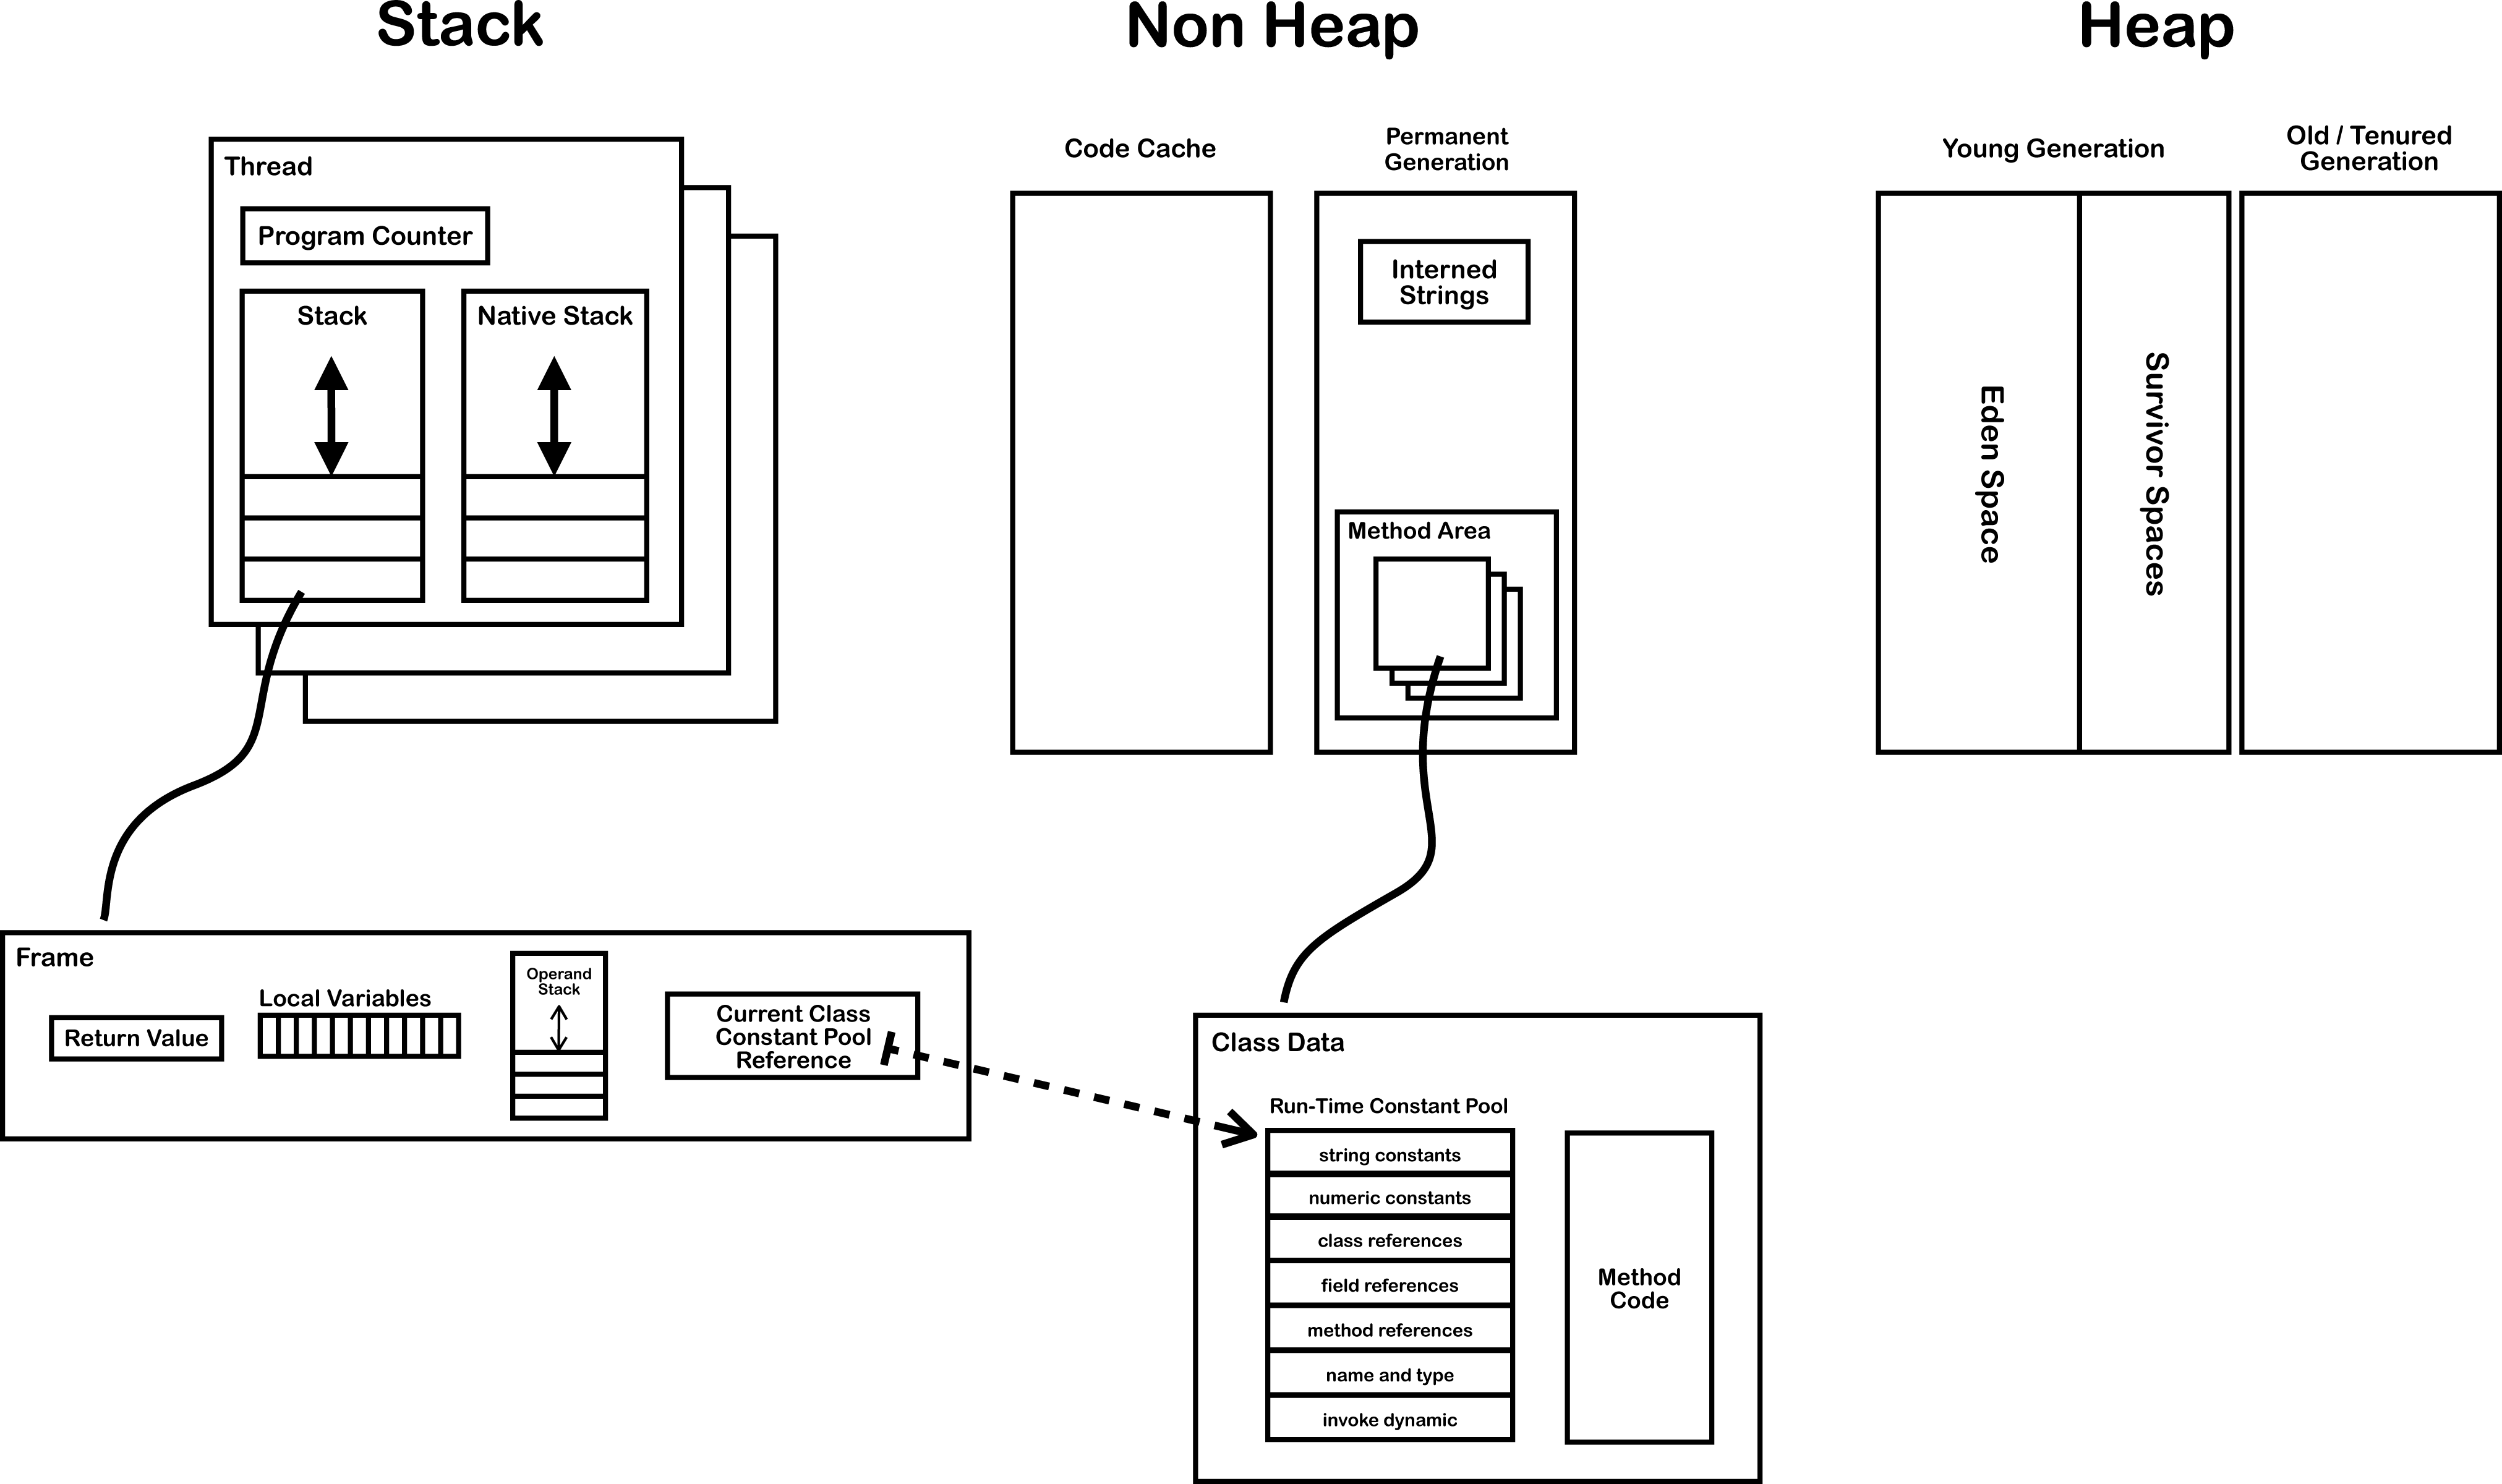
\includegraphics[scale=0.1]{obrazky/JVM_Internal_Architecture.png}
	\caption{Struktura Java paměti \cite{jvms-img}.}
	\label{obr-jvms-img}
\end{figure}

% =====================================================================================================================================================================================



\chapter{Analýza paměti}

Paměť je možné analyzovat za běhu programu nebo z jejího snímku -- reprezentace paměti v určitém okamžiku běhu programu.

\section{Analýza za běhu programu}
Během běhu programu lze analyzovat aktuální obsah paměti -- \zkratka{GC} koneckonců nedělá nic jiného. Problémem tohoto přístupu je ovšem dopad na výkon. I samotný \zkratka{GC}, ať už umožňující současný běh kódu nebo \textit{stop-the-world}, má výrazný dopad na výkon oproti jazykům či běhovým prostředím bez něj \cite{gc}. Navíc, běh \zkratka{GC}, stejně tak jako režie běhu samotného prostředí, jsou v drtivé většině případů v maximální možné míře optimalizovány, aby byl dopad na výkon samotného programu co nejmenší a jeho běh co nejrychlejší. Mohou využívat celou řadu nízkoúrovňových optimalizací, kterých -- v některých jazycích, včetně Javy -- dosáhnout prakticky nemůžeme. Z toho můžeme usoudit, že dopad analýzi paměti programu za jeho běhu by byl přinejmenším takový, jako dopad běhu \zkratka{GC}; pravděpodobně však výrazně vyšší. Stejně tak musíme uvažovat, že běh naší analýzy -- ať už pouze za účelem sběru dat pro pozdější zpracování -- bude výrazně složitější (či výkonově náročnější), než běh \zkratka{GC}.

Dalším důvodem pro vyhnutí se analýze za běhu programu je povaha řešeného problému a tedy implementovaného algoritmu. Protože potřebujeme provádět hloubkovou analýzu (všech či vybraných) objektů programu, jejich neustálá změna by tuto analýzu za běhu programu učinila nemožnou. Respektive bychom se nemohli vyhnout eventuálním falešně negativním či positivním hlášením -- to si jednoduše můžeme představit. Jestliže s každým cyklem analýzy zpracujeme jeden objekt a během toho dojde ke změně dat některého z dalších objektů, pak by algoritmus zahlásil při zpracování dalších objektů falečně pozitivní nález. V žádném časovém okamžiku neexistovaly dva objekty se stejnými daty, algoritmus by je tak přesto označil.


\begin{figure}[h]
	\centering
	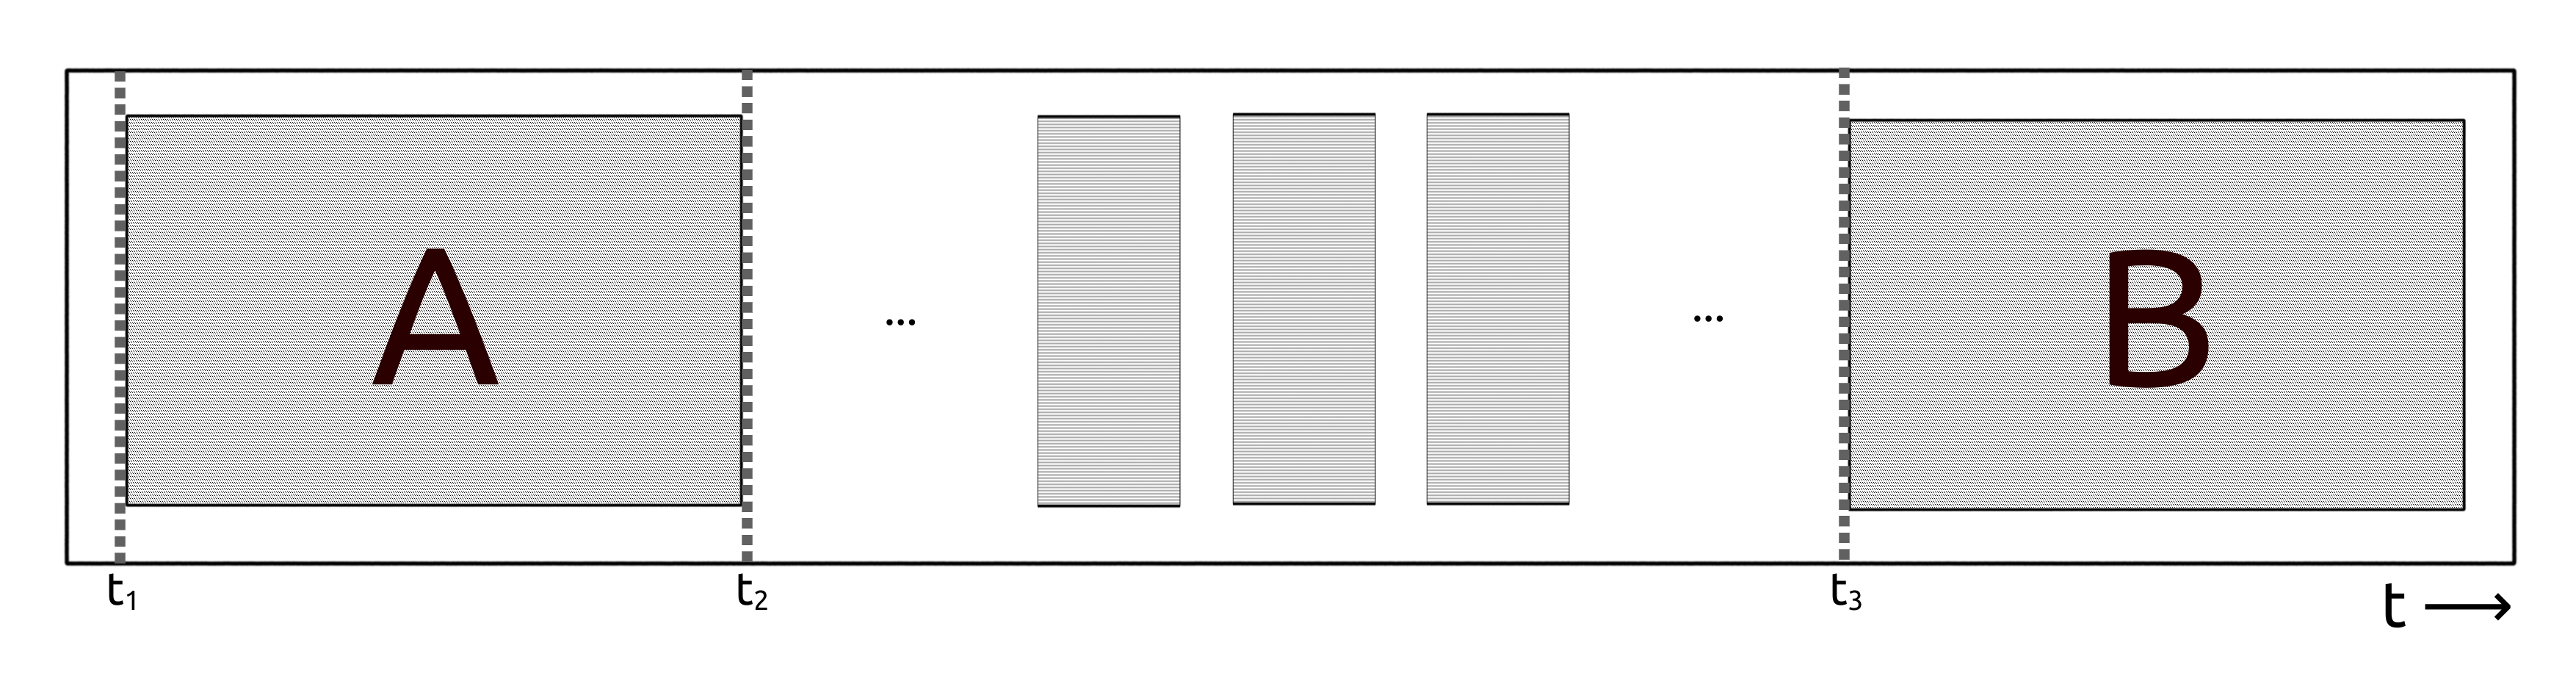
\includegraphics[scale=0.5]{obrazky/runtime-analysis.png}
	\caption{Problém analýzy paměti za běhu programu.}
	\label{obrRuntimeAnalysis}
\end{figure}



% =====================================================================================================================================================================================



\chapter{Optimalizace užití paměti}

Jak již bylo zmíněno v úvodu, využití paměti lze optimalizovat na několika úrovních. Vzhledem k tématu této práce se při uvažování optimalizací omezíme pouze na běžící Java aplkaci. Eliminaci případných zbytečných knihoven, frameworků a nástrojů se věnovat rovněž nemusíme. Analyzovat procentuální využití nabízených funkcí knihovny by mohlo být zajímavé, nicméně tento typ zbytečného užívání paměti nelze přímo označit za memory waste.

Můžeme tedy omezit samotné využití objektů -- zvážit, zda je potřebujeme, případně zda neexistuje vhodnější způsob či struktura pro jejich uchovávání. Jejich alokaci v paměti bychom rovněž meli omezit na nejkratší možnou dobu, po kterou si budeme jisti jejich využitím. Nicméně i zde je vhodné najít vhodný poměr mezi optimalizací a zbytečným úklidem objektu, který za několik okamžiků znovu budeme vytvářet.

Nejpřímějším způsobem optimalizace užití paměti se může jevit odstranění objektů, které už nejsou zapotřebí a nikdo je tedy nevlastní. Takové objekty nicméně nemusíme v naší optimalizaci uvažovat. O jejich uvolnění z paměti se postará \zkratka{GC}. Této vlastnosti jazyku tedy můžeme využít a nepotřebné objekty ručně odstraňovat -- nastavit je jako \texttt{null}. K jejich uvolnění dojde i při opuštění aktuálního prostoru -- oboru platnosti lokální proměnné. K takovému uvolnění nicméně nedochází přímo zapomocí analýzy \zkratka{GC}, ale díky uložení lokálních proměnných v zásobníku, z kterého jsou při opuštění bloku odstraněny.



% =====================================================================================================================================================================================



\chapter{Java Virtual Machine}
Program napsaný v Javě běží typicky v některé z implementací \zkratka{JVM}. \zkratka{JVM} je program, který slouží jako běhové prostředí pro uživatelský kód -- vykonává jeho instrukce a slouží tak jako prostředník mezi ním a operačním systémem (respektive jako interpret jeho kódu, který následně překládá do jiného jazyka, typicky strojového kódu dané architektury či platformy). \zkratka{JVM} je možné si představit jako virtuální počítač -- má vlastní instrukční sadu a na základě ní provádí operace nad pamětí. Díky tomu je možné jej, v případě potřeby, implementovat i jako CPU -- taková hardwarová implementace se nazývá \textit{Java procesor}. 

\zkratka{JVM} nemá ponětí o existenci Javy jako jazyku. Vidí pouze výsledek kompilace do bytecodu (viz dále), což je posloupnost operací z výše zmíněné instrukční sady. Jako analogii je možné zmínit instrukční sadu CPU a strojový kód -- CPU také netuší, jaký vyšší programovací jazyk je původcem strojového kódu, a při podobné implementaci kompilátoru dvou jazyků by to ani neměl šanci zjistit. Stejně tak se chová \zkratka{JVM} a bytecode -- ostatně existují i další jazyky na platformě \zkratka{JVM}, za všechny můžu jmenovat třeba populární Kotlin \cite{jvms-jvm}.

Některé implementace \zkratka{JVM} umožňují přímý překlad do strojového kódu bez potřeby interpretace, např. GraalVM \cite{graalvm}. V takovém případě hovoříme o tzv. \zkratka{AOT} přístupu, místo \zkratka{JIT} postupu implementovaného v moderních verzích častěji používaných \zkratka{JVM}, např. HotSpot od společnosti Oracle [TODO zdroj, že HS používá JIT].

\zkratka{JVM} se stará o načtení kódu ze souboru \texttt{.class}, dále o jeho verifikaci, spuštění a zároveň poskytuje tomuto kódu prostředí, v rámci kterého může běžet.

\section{Java Bytecode}
Java využívá dvoufázový překlad, tj. samotný zdrojový kód vytvořený programátorem je nejprve přeložen do \textit{bytecodu} (či česky bytekód). Bytecode je (či by měl být) platformě nezávislý soubor instrukcí, který následně \zkratka{JVM} vykoná v prostředí architektury a platformy, na které je spuštěn. To znamená, že zdrojový kód v jazyce Java (či kompatibilních jazycíc využívajících stejné prostředí, např. Kotlin), uložený typicky v souboru \texttt{.java}, je přeložen do bytecodu -- typicky s typu \texttt{.class}. Takové soubory je následně, obecně vzato, možné přenést na jinou platformu či architekturu a jestliže se zde nachází kompatibilní \zkratka{JVM}, je možné jej bez úpravy na daném systému vykonat a tedy program spustit. Bytecode se může přenášet formou klasických jednotlivých souborů \texttt{.class} či v zabalené formě, tj. archiv typu \texttt{.jar} (což je de facto pouze zip archiv s předem danou strukturou a volitelně přidanými informacemi -- manifestem, metadaty, podpůrnými soubory (\textit{resources})).

\section{Class loader}
Jak už jsem zmínil, \zkratka{JVM} se stará o načítání dat ze souboru \texttt{.class}. Konkrétně se o toto načítání stará objekt nazvaný \textit{class loader}. Ten, typicky, načítá třídy ze souborového systému, konkrétně z cesty (nebo z více cest) definované v proměnné \texttt{CLASSPATH}. Nicméně, díky tomu, že koncept class loaderů je poměrně abstraktní, je možné načítat třídy například přes síť, z paměti nebo je dynamicky vytvářet za běhu programu dle potřeby. Každá načtená třída (konkrétně objek typu \texttt{Class}) obsahuje referenci na objekt class loaderu, který ji zavedl do programu -- konkrétně jej lze obdržet pomocí metody \texttt{getClassLoader()} (v případě primitivních typů vrací \texttt{null}). \texttt{ClassLoader} je definovaný jako abstraktní třída, lze tedy definovat vlastní loadery dle potřeby. 

Pokud \texttt{JVM} narazí na třídu, podívá se do setu načtených tříd. Jestliže se tam nachází, vezme ji (instanci třídy \texttt{Class}) a použíje. Pokud ne, požádá o její načtení. Systém class loaderů funguje na principu delegování v následujícím pořadí (typicky, pokud jej neupravíme), jak zobrazuje obrázek \ref{obr-class-loader} \cite{class-loader} \cite{class-loader-hierarchy}. V případě, že třídu žádný z boot loaderů nenalezne, je produkována výjimka \texttt{ClassNotFoundException}. 

\begin{enumerate}
	\item Aplikace požádá \textit{Application class loader} o načtení třídy.
	\item Ten zavolá \textit{Extension class loader}.
	\item \textit{Extension class loader} zavolá \textit{Bootstrap class loader}.
	\item \textit{Bootstrap class loader} funguje v rámci výchozích \textit{JDK} a \textit{JRE} knihoven. Pokud třídu nalezne, tak ji vrátí. V opačném případě volá zpět \textit{Extension class loader}.
	\item \textit{Extension class loader} se podívá v rámci rozšíření \textit{ext} Javy. V případě neúspechu volá \textit{Application class loader}.
	\item \textit{Application class loader} načítá třídy z \texttt{CLASSPATH} (a třídy specifikované v Manifestu atd.)
\end{enumerate}

\begin{figure}[h]
	\centering
	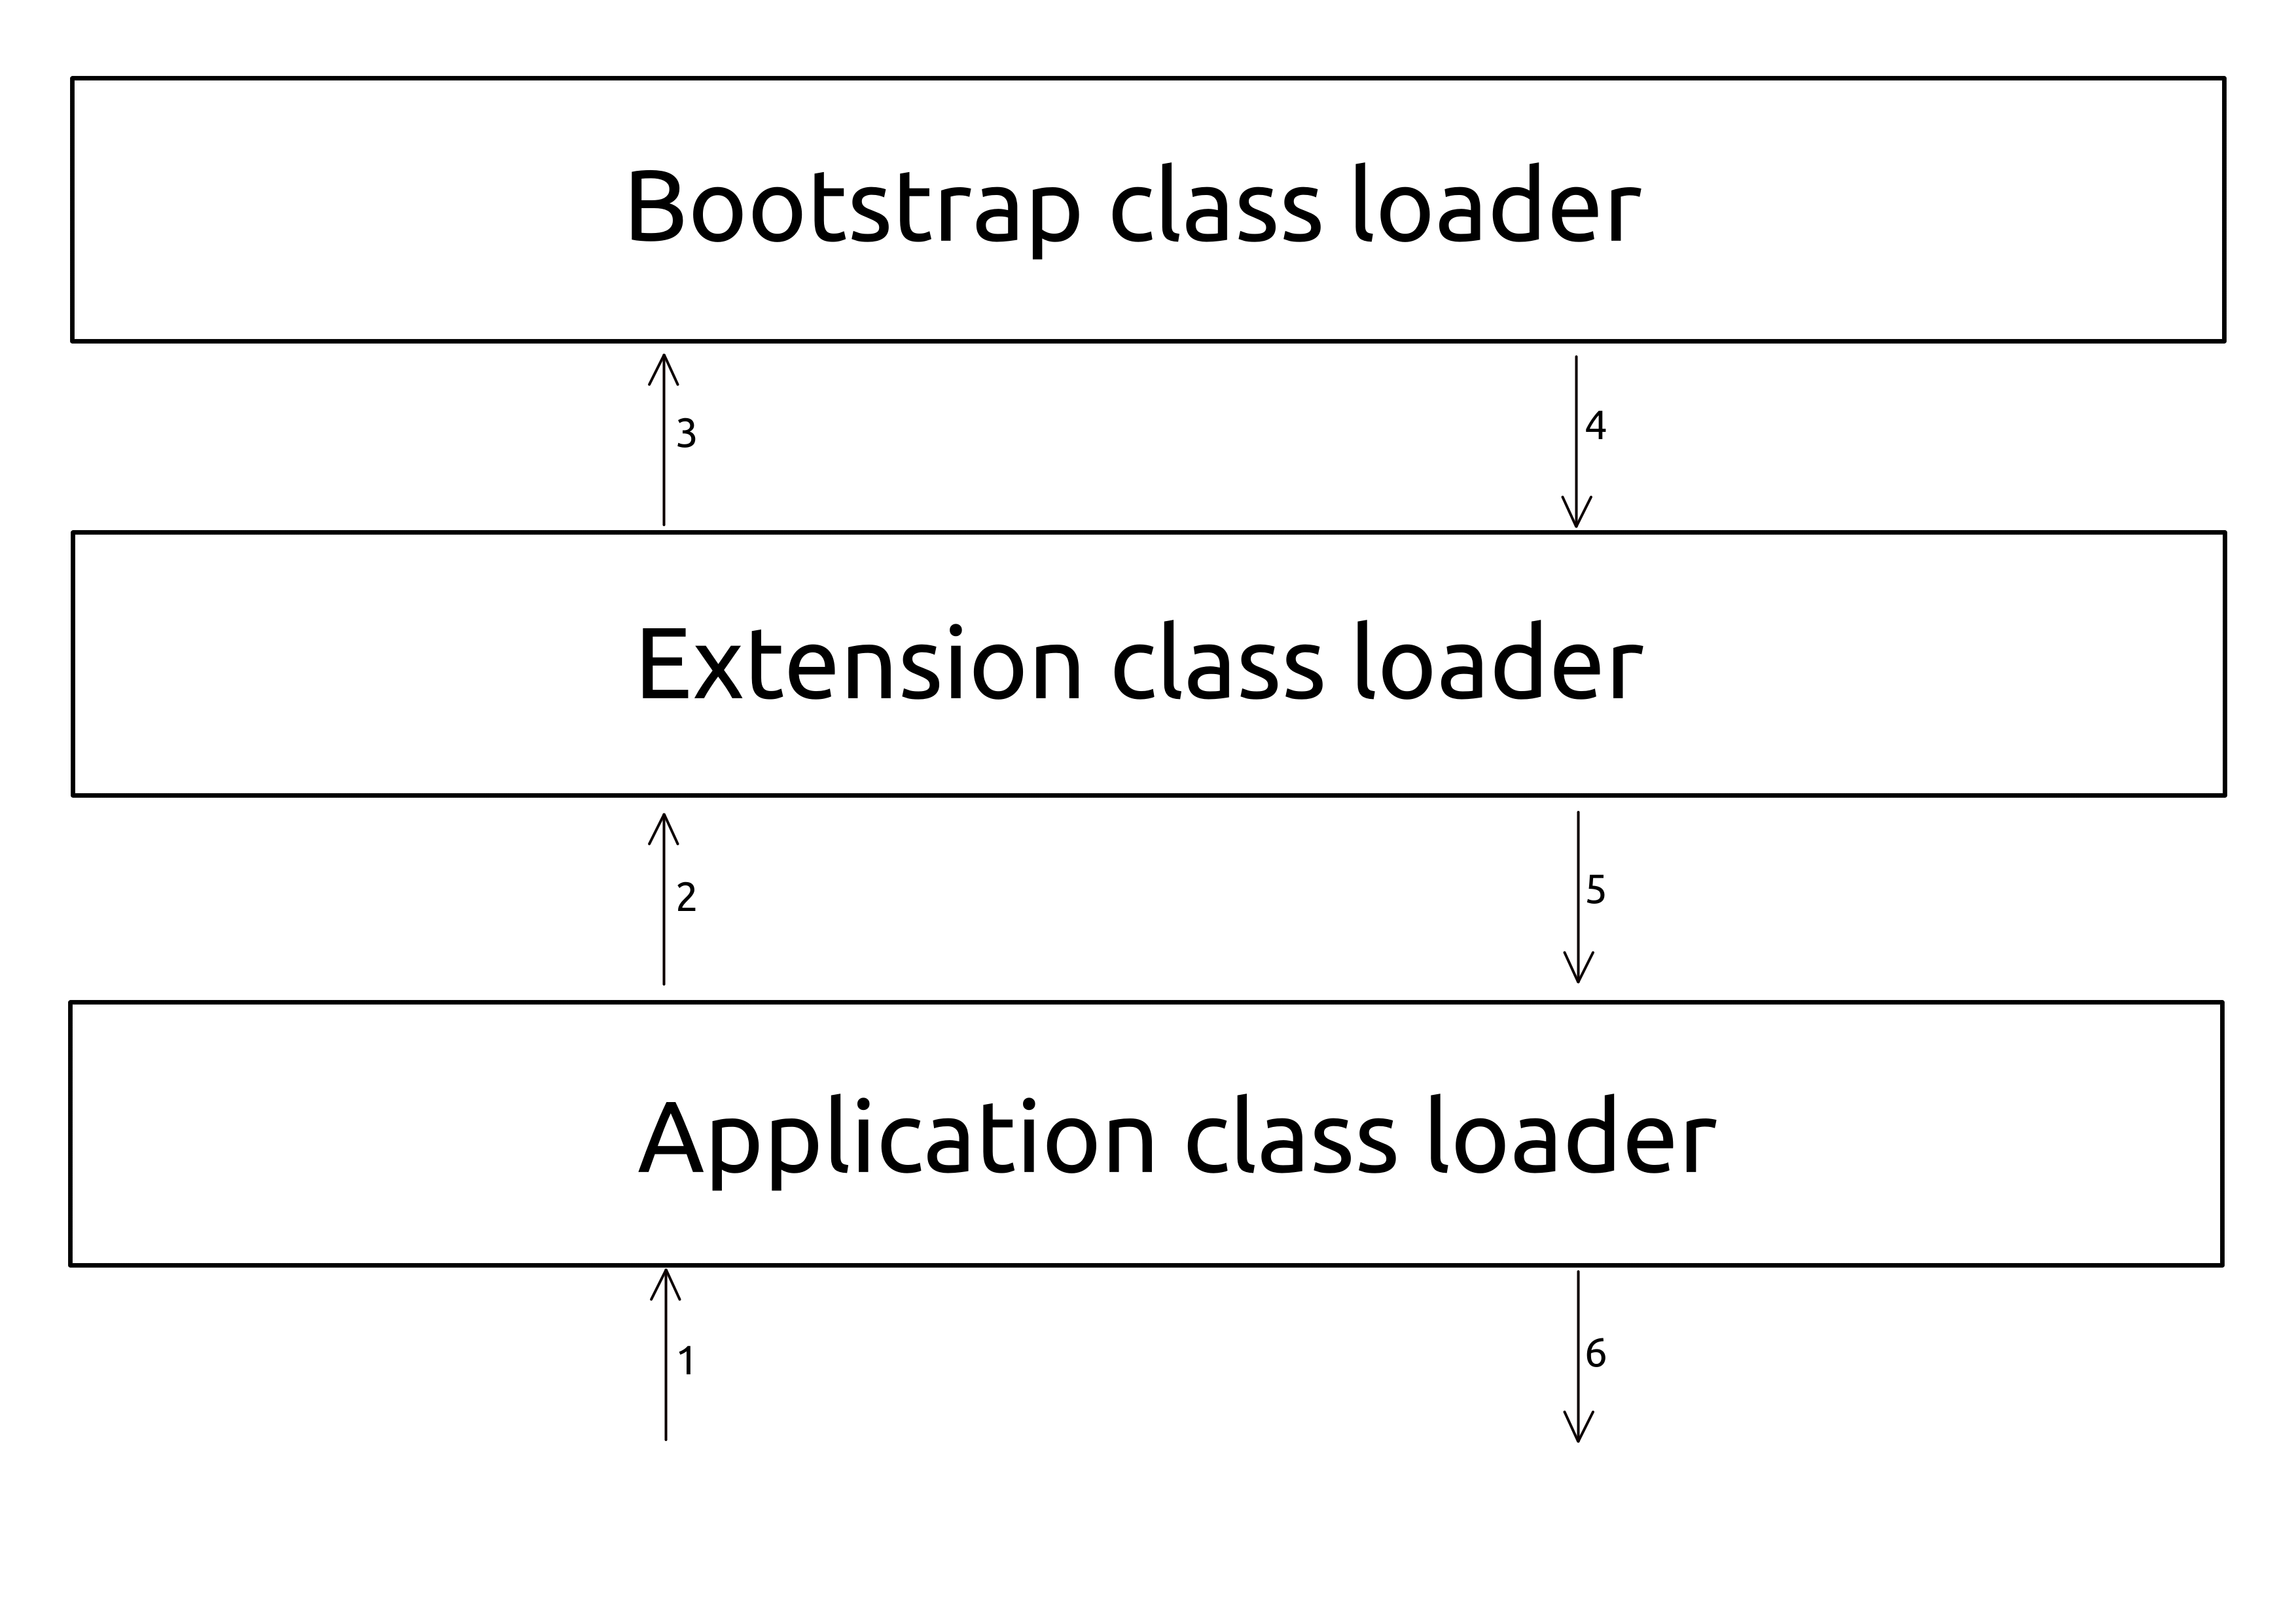
\includegraphics[scale=0.5]{obrazky/class-loader.png}
	\caption{Postup volání hierarchie class loaderů.}
	\label{obr-class-loader}
\end{figure}

% =====================================================================================================================================================================================



\chapter{Správa a struktura Java haldy}
\label{memory-management}

Paměťovému modelu v Javě se věnuje \textit{JSR-133}, nicméně přesně nespecifikuje konkrétní rozdělení paměti a způsob jejího přidělování a uvolňování. Následný popis se tedy věnuje implementaci od společnosti Oracle – HotSpot. Zde je paměť rozdělena na 2 logické celky – \textit{young generation space} a \textit{old generation space}. Tato paměť, tedy halda, je rozdělena pouze v rámci JVM a následně je mapována na skutečnou fyzickou paměť \cite{jsr133}.

Young generation space, tedy doslova “prostor mladé generace”, je dále rozdělen na \textit{eden space} a prostory \textit{S0} a \textit{S1}. Eden space slouží k vytváření nových instancí objektů, je zde tedy vyhrazena část paměti nově vytvořenému objektu. Pokud v tomto prostoru není volno, proběhne uvolnění paměti (viz dále) přesunutím některých objektů do S0. Každý takový objekt obsahuje informaci o tom, kolik takových uvolnění daný objekt \uv{přežil}.

Po určitém počtu takových přežití (či jinak také povýšení) je objekt přenesen do objektů staré generace, konkrétně \textit{Tenured space}.

Toto rozdělení objektů do jednotlivých prostorů se jeví jako zbytečná komplikace, má však řadu výhod. První z nich je rychlost – nejvíce operací uvolnění je prováděno právě nad eden spacem, který je z prostorů nejmenší. Dále jsou tak objekty rozdělovány do skupin s podobnou charakteristikou (podobný věk, podobný počet a styl referencí apod.), na kterými je poté možné spustit rozdílné, pro dané skupiny specifické algoritmy pro jejich uvolnění.

\section{Garbage collection}
	Spuštění \zkratka{GC} v Javě nelze vynutit ručně. Systému lze \textit{doporučit} jeho exekuci voláním metody \texttt{System.gc()}; \zkratka{JVM} se tím ale nemusí řídit a toto volání jednoduše ignorovat \cite{javagc}. 

I v Javě můžeme narazit na problém úniků paměti, tzv. \textit{memory leaků}. Typicky se tento problém týká nízkoúrovňových jazyků typu C, nebo takových jazyků, kde je správa paměti v kompletní kompetenci autora programu. Často dojde k \uv{zapomenutí} některého ukazatele. Jeho smazáním se paměť stává nedostupnou a protože v daném jazyku není \zkratka{GC}, bude uvolněna teprve ukončením programu -- operačním systémem samotným. Toto chování je nebezpečné, protože pokud program poběží dlouhou dobu a bude alokovat paměť bez jejího následného uvolnění, dříve nebo později narazí na limit kladený ze strany operačního systému. Rovněž může jeho provozování být nepříjemné pro provozovatele programu, protože i když jeho běh operační systém neukončí, program bude zabírat zbytečně velké množství paměti.

Ve spojení s \zkratka{GC} by tedy nemělo k únikům paměti typicky dojít. V Javě k nim může dojít především při nedůsledném používání vlastních zavaděčů tříd -- \textit{class loaderů}. Za únik paměti můžeme rovněž považovat neuzavřený popisovač otevřeného souboru, databáze či jiného zdroje. Pokud k němu ztratíme přístup, např. po vyhození výjimky bez uzavření tohoto popisovače v bloku \texttt{catch} či lépe \texttt{finally}, ztrácíme tím, spolu s popisovačem, i menší množství paměti. Při častějším výskytu problému ale v tomto případě pravděpodobně narazíme na horní limit popisovačů Javy či operačního systému -- ani tento zdroj není neomezený.

TODO popis různých implementací GC v Javě?

\section{Heap Dump}
\textit{Heap dump} je textová nebo binární reprezentace paměti, kterou je možné uložit na disk a zachycuje aktuální stav aplikace. Při vytváření je činnost aplikace pozastavena. Dump je možné následně analyzovat a dále zpracovávat, je tak možné prozkoumat vnitřní stav aplikace v určitém bodě a např. řešit příčiny neočekávaného chování. 

\subsection{Vytvoření dumpu}
Prostředků k vytvoření dumpu je několik. Při správném nastavení (pomocí parametru \texttt{HeapDumpOnOutOfMemoryError}) k němu dojde při nedostatku paměti zcela automaticky. Mezi manuální způsoby vytvoření patří primárně nástroj \textit{JMAP}, který je publikován spolu se standardní distribucí Oracle JVM. Při použití tohoto nástroje je nutné naprosto přesně dodržet číslo verze JMAP a JRE, pod kterým cílová aplikace běží – dumpování rozdílných verzí není podporováno, je nutné dodržet rovnost verzí (major, minor i update).

Mezi další způsoby vytvoření dumpu patří různé nástroje, debuggery a profilery typu Eclipse MAT, VisualVM nebo Java Mission Control (viz dále). Výhodou těchto nástrojů je, že dokáží zvládnout vytváření dumpu i napříč verzemi a dokonce implementacemi (z Oracle JDK na OpenJDK apod.)

Další možnost je využít některou z knihovních funkcí a vytvářet tak dump programově. Zde je možné využít např. MBeans. Nízkoúrovňovou možností je poté například použití Unixového nástroje \textit{gcore}, respektive \textit{GDB}, který se postará o vytvoření dumpu paměti procesu (pod daným \zkratka{PID}), tzv. \textit{core dump}. Z něj lze memory dump vyextrahovat. Pokročilejší nástroje typu VisualVM umí pracovat i napřímo s core dumpem.

\subsection{Vztah dumpu vůči paměti procesu}
Heap Dump přímo odpovídá části paměťového prostoru procesu, resp. heapu. Je tedy přímým otiskem části fyzické paměti tak, jak je uložena, v určitém časovém okamžiku. Toto je možné si experimentálně ověřit -- jak bylo zmíněno výše, z otisku fyzické paměti je možné heap dump získat. Je tedy evidentní, že při jeho vytvoření některým z výše uvedených způsobů nedochází k žádným úpravám a snímek je vytvořen \uv{tak jak je}. 

\begin{figure}[h]
	\centering
	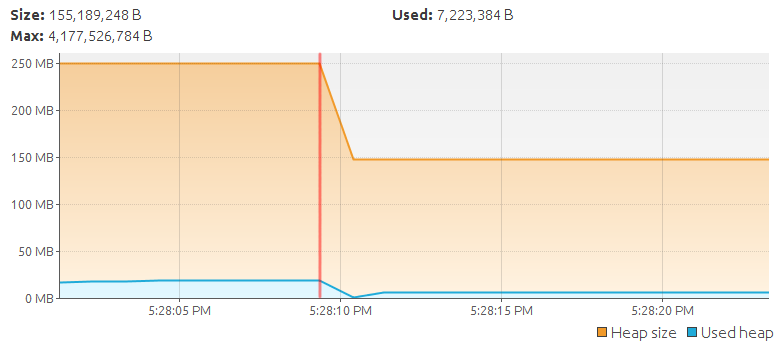
\includegraphics[scale=0.5]{obrazky/heapdump-performed.png}
	\caption{Využití paměti a provedení garbage kolekce před vytvořením dumpu (červeně).}
	\label{obr1}
\end{figure}

\section{Zpracování dumpu}
Při zpracování dumpu je nutné zohlednit fakt, že je vyexportovaný kompletní paměťový prostor [TODO zdroj] a nachází se zde tedy i data objektů, které nás nutně nemusí zajímat – typicky knihovny nebo objekty Javy. Toto je možné zohlednit a filtrovat na základě jmenného prostoru (namespace), do kterého objekt patří.

Pro práci nad heapem  (typicky ve formátu HPROF) je možné využít některou z implementací dotazovacího jazyku OQL (Object Query Language).



% =====================================================================================================================================================================================



\chapter{Existující nástroje pro analýzu heapu}

Analýza dumpu -- ať už manuální či automatická -- je využívána v případech, kdy nám debugování na úrovni kódu už nestačí a potřebujeme se podívat, jakým způsobem se program chová na pozadí. Rovněž je jeho analýza vhodná v okamžiku, kdy dojde k pádu (zejména v důsledku nedostatku paměti), kdy chceme zjistit příčinu pádu \uv{post mortem}. Můžeme tak odhalit problematické místo v programu a podrobná analýza nám tak umožní problém opravit.

\section{Eclipse MAT}
IBM Eclipse Memory Analyser Tooling je open source nástroj pro analýzu Java paměti. Po spuštění umožňuje otevřít již vygenerovaný dump Java heapu, umí jej ale i vytvořit. V rámci analýzy nabízí 2 konkrétní volby – analýzu memory leaků a memory bloatu – tj. neefektivního využití paměti a zbytečného plýtvání. 

MAT se analýzou memory bloatu přibližuje zamýšlenému výsledku této práce, bohužel ale nenabízí kompletní funkcionalitu v této oblasti. Omezuje se pouze na efektivní práci s řetězci (kterou už obsahuje Java, respektive JVM v základu, viz TODO) a dalšími základnímu typy, např. Map. Cílem práce je ale zpracování všech možných objektů, tato funkcionalita by se tak dala případně rozšířit.

Nástroj je založený na platformě Eclipse RCP (Rich Client Platform), respektive OSGi. Díky tomu je poměrně snadno rozšiřitelný, což je ale vyváženo velkým rozsahem aplikace, který vývoj a rozšíření naopak lehce komplikuje. Buildovacím nástrojem je zde Maven.

\section{VisualVM}
Open source profiler pro Java platformu. Patří mezi nejpoužívanější profilery, respektive nástroje pro analýzu výkonu v Javě.

Po spuštění nabízí klasické funkce typické pro profilery, tj. využití paměti, zatížení CPU, počet objektů a vláken a podobné statistiky. Kromě toho obsahuje celou řadu dalších funkcí, jako provedení garbage kolekce (její vyžádání, explicitně vyvolání GC není možné) nebo vytvoření heap dumpu.

Požadovanou funkcionalitu VisualVM v zásadě neposkytuje, umožňuje pouze k nahlédnutí tabulku s informacemi – kolik bylo vytvořeno instancí jaké třídy, respektive jimi okupovanou paměť. V programu využít podporu pro OQL syntaxi, což je možné využít, nicméně tento přístup nelze považovat za dostačující.

Pro build je využíván nástroj Ant a v současné době je vyžadována Java verze 7 a vyšší.

\section{Java Mission Control}
Nástroj poskytovaný přímo spolu s distribucí Oracle JVM od verze 7 (konkrétně 7 Update 40 – 7u40), což je jeho výhodou. Mezi jeho možnosti patří např. využití paměti jednotlivými součástmi Java paměti a také umožňuje zobrazit jednotlivé instance objektů, nicméně neumožňuje jejich další analýzu.

\section{JProfiler}
Komerční profiler, přesto velice používaný. Standardní licence stojí v době psaní 409 euro, akademická potom 179 euro. Je možné zažádat o licenci pro open source produkty, nicméně ta je podmíněna již vydanou verzí a existující webovou stránkou, což činí jakékoliv použití tohoto profileru v rámci práce nepraktickým. Profiler je používán především v komerční sféře, díky svým možnostem a dle výše uvedeného testu i nejvyšší úspěšností v odhalování bugů.

\section{JHAT}
Nástroj, který je přímou součásti distribuce Oracle JVM od verze 6. Nebyl nikdy oficiálně podporován a od počátku byl označen jako experimentální nástroj, z těchto důvodů byl tedy v Javě 11 naprosto odstraněn \cite{jep241}\cite{java11migration}. V rámci verzí Javy, které jej obsahují, ho lze využít jako \zkratka{CLI} aplikaci, která dokáže dump vytvoření pomocí např. \textit{JMAP} otevřít. Následně vytvoří webový server, jehož prostřednictvím poskytuje data získaná ze zpracovaného dumpu. Tato data je možné si poté zobrazit pomocí webového prohlížeče; zajímavým příkladem možného využití je následné rozparsování těchto dat jakožto formátu HTML a jejich další využití. Program je tedy možné využít jako prostředníka pro zpracování \cite{jhat}. Kromě \uv{prostého} zobrazení webové stránky umí \textit{JHAT} rovněž poskytovat zpracování pomocí jazyka \zkratka{OQL}.

\section{\zkratka{OQL}}
\zkratka{OQL} zmíním i jako samostatný způsob zpracování. Jedná se o jazyk, který slouží pro obecnou manipulaci s objekty, resp. s objektovými dokumenty \cite{odmgoql}\cite{oql}. Na první pohled si nelze nevšimnou jeho podobnosti s dotazovým jazykem SQL. Neomezuje se tedy pouze na zpracování Java heapu (či obecně paměti), ale je standardem, který pro tento účel lze využít. Z toho je možné usoudit, že standard jako takový pro zpracování nestačí -- je nutné využít některou z jeho implementací, která takové rozhraní přístupu k Java heapu umožňuje. Jednou z nich je právě výše zmíněný \textit{JHAT}.

V příkladu \ref{oql}.

\begin{lstlisting}[caption={Příklad OQL}, label={oql}, frame={single}, language={SQL}]
select s 
from java.lang.String s 
where s.value.length >= 100
\end{lstlisting}



% =====================================================================================================================================================================================



\chapter{Možnosti analýzy}
Rovnost dvou či více objektů se dá definovat a zjišťovat různými způsoby. Je ale nutné si uvědomit, že v nejhorším případě, tj. pokud chceme najít všechny nadbytečné kopie každého objektu, je složitost této operace $O(2^n)$. Bylo by tedy vhodné se zamyslet, zda neexistuje způsob, jak počet porovnání snížit, případně navrhnout jednoduchou heuristiku, která by dokázala rychle ohodnotit, zda má vůbec smysl pokračovat v podrobnějším porovnání. V následujících případech tedy uvažujme objekty $A$, $B$, jejich třídy $C_A$ a $C_B$ a proměnné obou instancí $F_A^0..F_A^n$, respektive $F_B^0..F_B^n$.

První nápovědou samozřejmě může být porovnání tříd obou objektů -- $C_A$ a $C_B$. Pokud platí $C_A = C_B$, zřejmě má smysl se porovnáváním dále zabývat. V případě jejich nerovnosti není ale možné další porovnání zavrhnout, porovnat je nutné (či možné) i jejich rodiče. Definujeme-li tedy funkci pro zjištění přímého rodiče $P(C)$, potom rovnost objektů lze vyjádřit jako
    $$ E(C_A, C_B) \Leftrightarrow C_A = C_B \vee E(P(C_A), C_B) \vee E(C_A, P(C_B)).$$    
Samozřejmě je nutné definovat i zastavovací podmínku, v případě Javy by tedy jeden z parametrů nesměl být třída typu \textit{Object}. Formálně je tedy možné tuto rovnost definovat jako
	$$ E(C_A, C_B) = P_c(C_A) \cap P_c(C_B) \notin \emptyset,$$
kde $P_c(C)$ je množina třídy samotné a všech jejich rodičů bez “univerzálního předka” všech tříd, v tomto případě \textit{Object}:
	$$ P_c(C) = \{C, P(C), P(P(C)), \dots, Object\} \setminus Object. $$
% Nejjednodušší cestou je prosté porovnání hodnot jednotlivých


\chapter{Analýza a implementace}
